\documentclass[a4paper]{report}
\usepackage[margin=1.5in]{geometry}

\usepackage[utf8]{inputenc}
\usepackage[T1]{fontenc}
\usepackage{textcomp}
\usepackage[spanish]{babel}
\decimalpoint

\usepackage{csquotes}
\usepackage[sorting=none]{biblatex}
\addbibresource{refs.biblatex}

\usepackage{amsmath, amssymb}
\usepackage{amsthm}
\usepackage{bm}
\usepackage{braket}

\usepackage{graphicx}

\usepackage{hyperref}
\hypersetup{
    colorlinks,
    citecolor=red,
    filecolor=black,
    linkcolor=blue,
    urlcolor=black
}

\DeclareMathOperator{\R}{\mathbb{R}}
\DeclareMathOperator{\C}{\mathbb{C}}
\DeclareMathOperator{\N}{\mathbb{N}}
\DeclareMathOperator{\Z}{\mathbb{Z}}

\let\H\relax
\DeclareMathOperator{\H}{\mathcal H}
\DeclareMathOperator{\Sz}{\mathcal S}

\DeclareMathOperator{\dom}{Dom}
\DeclareMathOperator{\prob}{Prob}
\DeclareMathOperator{\id}{id}
\DeclareMathOperator{\Tr}{Tr}
\DeclareMathOperator{\Op}{Op}
\DeclareMathOperator{\W}{W}
\DeclareMathOperator{\F}{\mathcal{F}\!}

\newtheorem{definition}{Definición}
\newtheorem{theorem}{Teorema}
\newtheorem{proposition}{Proposición}
\newtheorem{lemma}{Lema}
\newtheorem{corollary}{Corolario}
\newtheorem{example}{Ejemplo}
\newtheorem{axiom}{Axioma}
\newtheorem{remark}{Observación}

\hfuzz=50pt

\title{Funciones de Wigner en el Espacio de Fase Discreto}
\author{Ernesto Camacho Ramírez}

\begin{document}
  \maketitle

  \tableofcontents

  \chapter{Introducción}

  El número de elementos de un conjunto general de
  operadores cuánticos unitarios sobre estados de $n$-qudit
  generalmente crece exponencialmente con $n$. Una excepción
  importante a ésta regla involucra el conjunto de
  operadores de Clifford que actúan sobre estados
  estabilizadores. Éstos estados juegan un papel importante
  en la corrección de errores cuánticos
  \cite{gottesmanHeisenbergRepresentationQuantum1998} y son
  cerrados bajo la acción de las compuertas de Clifford. La
  simulación eficiente de dichos sistemas con una
  computadora clásica se demostró con el algoritmo tableau
  de Aaronson y Gottesman \cite{
    aaronsonImprovedSimulationStabilizer2004,
  gottesmanHeisenbergRepresentationQuantum1998} para qubits
  ($d=2$). La busqueda de un explicación de por qué un
  algoritmo tan eficiente es posible para la simulación de
  circuitos de Clifford ha sido un objeto de mucho estudio
  \cite{gottesmanFaultTolerantQuantumComputation1999,
    howardContextualitySuppliesMagic2014,
  mariPositiveWignerFunctions2012}. El progreso reciente ha
  sido resultado del trabajo de Wooters
  \cite{woottersWignerFunctionFormulationFiniteState1987},
  Eisert \cite{mariPositiveWignerFunctions2012}, Gross
  \cite{grossHudsonTheoremFinitedimensional2006} y Emerson
  \cite{howardContextualitySuppliesMagic2014}, quienes han
  formulado una nueva perspectiva basada en los espacios de
  fase discretos de estados y operadores en espacios de
  Hilbert finitos, utilizando funciones discretas de Wigner.
  Se ha demostrado que los estados estabilizadores tienen
  funciones de Wigner discretas definidas positivas y que
  los operadores de Clifford son mapeos definidos positivos.
  Esto implica que los circuitos de Clifford son simulables
  eficientemente en computadores clásicas. En sistemas de
  dimensiones impares, se ha demostrado que los estados
  estabilizadores son análogos discretos a los estados
  gaussianos en sistemas continuos
  \cite{grossHudsonTheoremFinitedimensional2006} y se ha
  demostrado que las compuertas del grupo de Clifford tienen
  Hamiltonianos armónicos subyacentes que conservan los
  puntos discretos del espacio de fase
  \cite{kociaSemiclassicalFormulationGottesmanKnill2017}.
  Esto significa que los circuitos de Clifford se pueden
  expresar mediante integrales de trayectoria truncadas en
  el orden $\hbar^{0}$ y por lo tanto son expresamente
  clásicos
  \cite{kociaSemiclassicalFormulationGottesmanKnill2017,
  kohComputingQuopitClifford2017}.

  En este trabajo, buscamos construir, de una manera
  explícita, los operadores \textit{puntuales} de fase
  discretos (núcleos de la transformación de Wigner) para
  qubits y qutrits. Estrictamente hablando, buscamos la
  construcción \textit{estándar}
  \cite{woottersWignerFunctionFormulationFiniteState1987} y
  \textit{no estandar} (contribución del trabajo) de los
  núcleos que permitan dos formas de la función de Wigner,
  utilizando conjuntos de bases no equivalentes bajo
  transformaciones unitarias. La motivación para realizar
  éste trabajo es que, los núcleos que no son equivalentes
  conservan la propiedad tomográfica básica, lo que permite
  expresar la función de Wigner de cualquier estado como una
  combinación lineal de probabilidades medidas y la
  inequivalencia conduce a la posibilidad de encontrar
  estados no estabilizadores con funciones de Wigner no
  negativas, lo que contrasta con resultados previos para el
  caso discreto
  \cite{grossHudsonTheoremFinitedimensional2006,
  galvaoDiscreteWignerFunctions2005,
  cormickInterferenceDiscreteWigner2006}.

  \chapter{Preliminares}

  Para poder estudiar la función de Wigner discreta es
  necesario presentar la función de Wigner en el caso
  continuo. Para ésto requerimos un conocimiento básico de
  la mecánica cuántica, la cual es una teoría física que
  nació debido a la incapacidad de la mecánica clásica de
  explicar algunos fenómenos físicos que se observaban a
  nivel atómico. A diferencia de la mecánica clásica, la
  teoría cuántica es probabilística naturalmente y sus
  formulaciones matemáticas son bastante distintas. En la
  mecánica clásica, cuando se fija un estado de un sistema
  físico, el valor especificado por un observable (algo se
  puede medir del sistema) está completamente determinado.
  En la mecánica cuántica ésto ya no es cierto, los
  observables solo nos brindan distribuciones de los
  posibles valores. Antes de plantear los principios de la
  mecánica cuántica, repasamos rápidamente el concepto del
  espacio de fase en la mecánica clásica, ya que unas de las
  ideas principales de la distribución de Wigner es vincular
  éstas dos teorías físicas.

  \section{La mecánica clásica y el espacio de fase}

  El concepto del espacio de fase es una herramienta de la
  mecánica clásica, la cual describe la evolución temporal
  de un sistema físico. Dicho de una manera muy sencilla, la
  mecánica clásica estudia partículas y sus trayectorias,
  las cuales se rigen de acuerdo a las leyes de Newton.  Se
  considera que la partícula se `mueve' en un espacio
  euclideano, es decir, su \textit{posición} está dado por
  $\bm{x} = (x_1,\ldots,x_n) \in \R^{n}$. El
  \textit{momentum} es una cantidad dada por $p_j = m \dot
  x_j$, donde $\bm{\dot x}$ es la derivada respecto al
  tiempo de la posición, es decir, la velocidad de la
  partícula, y $m$ es la \textit{masa} de la partícula. Las
  cantidades que uno desea medir de nuestro sistema físico
  se les llama \textit{observables}, y en la mecánica
  clásica, son las funciones continuas que tienen como
  argumentos las cantidades $\bm{x},\bm{p}$ y $m$. Ejemplos
  de ellos son el momentum, la energía cinética, la energía
  potencial, etc. La función de energía más usual es la que
  está dada como la suma de la \textit{energía cinética} y
  \textit{energía potencial}:
  \begin{equation}
    H(\bm{x},\bm{p})
    = \frac{1}{2m} \sum_{j=1}^{n} p_j^2 + V(x).
  \end{equation}
  A la energía del sistema se le conoce como el
  \textit{Hamiltoniano}.  Utilizando ésta función de
  energía, la ley de Newton nos brinda las ecuaciones de
  movimiento de la partícula en cuestión:
  \begin{equation}
    \frac{dx_j}{dt}
    = \frac{\partial H}{\partial p_j},
    \quad
    \frac{dp_j}{dt}
    = -\frac{\partial H}{\partial x_j}.
  \end{equation}
  Expresada como un sistema de ecuaciones diferenciales, a
  la ley de Newton se le conoce como las \textit{ecuaciones
  de Hamilton}.  

  Con ésto, es natural representar el estado del sistema
  clásico considerando el par $(\bm{x},\bm{p})$. Al espacio
  $\R^{2n}$ correspondiente le llamamos el \textit{espacio
  de fase}. A las soluciones de las ecuaciones de Hamilton
  se les conoce como \textit{trayectorias}, y son curvas que
  viven en el espacio de fase.
  \begin{definition}
    El espacio de fase de una partícula que se mueven en
    $\R^{n}$ es $\R^{2n}$, considerado como el conjunto de
    las $(2n)$-tuplas de la forma
    \[
      \left(
        x_1, \ldots, x_n, p_1, \ldots, p_n
      \right),
    \] 
    donde $x_j$ y $p_j$ son elementos de $\R$.
  \end{definition}

  Cabe mencionar que el tratado moderno de la mecánica
  clásica está fundamentado en la geometría diferencial de
  las variedades simplécticas
  \cite{mcinerneyFirstStepsDifferential2013}, en donde el
  espacio de fase se define como el espacio cotangente del
  espacio de configuraciones $T^{*} \R_x \cong \R_x \times
  \R_p$, donde el espacio de configuraciones  $\R_x$ es el
  espacio de posición y el $\R_p$ es el espacio del
  momentum.  Para nuestros objetivos basta con desginar el
  espacio de fase como el espacio $\R^{2n}$.

  Notemos que por el momento no ha surgido ninguna
  interpretación probabilística en la mecánica clásica, pues
  es una teoría determinística. Dado que la teoría cuántica
  es probabilística, es natural preguntarnos ¿qué
  características de la mecánica clásica serían deseables en
  la teoría cuántica? y ¿qué beneficios habría en hacer un
  vínculo entre la mecánica clásica y la cuántica?
  \cite{schroeckQuantumMechanicsPhase1996}, especialmente
  cuando sabemos que la teoría cuántica (y sus derivados) es
  nuestra teoría más precisa. Un esfuerzo por vincular las
  descripciones clásicas y cuánticas del mundo es la
  representación de Wigner-Weyl de la mecánica cuántica.
  Ésta es una formulación que intenta usar la noción del
  espacio de fase en la dinámica cuántica y la idea básica
  es la construcción de \textit{cuasi-distribuciones}
  real-valuadas que representan a los sistemas cuánticos.

  \section{La mecánica cuántica}

  La teoría cuántica ha tomado distintas direcciones despues
  de su concepción en los años viente y existen distintas
  formulaciones matematicamente equivalentes que surgieron
  despues de las teorias iniciales de Schrödinger (mecánica
  de ondas) y de Heisenberg (mecánica matricial).  La más
  común hoy en dia es la formulación en el espacio de
  Hilbert, la cual fue desarrollada de manera rigurosa por
  Von Neumann en 1932.  La segunda formulación más común,
  especialmente en la teoría cuantica de campos, es la
  formulación de la integral de trayectoria de Feynman
  desarrollada en 1948.  Otra formulación, de particular
  interés para nuestro trabajo, es la formulación en el
  espacio de fase, que tiene sus inicios en 1932 por Wigner,
  pero que solo fue desarrollada como una descripción
  completa de la mecánica cuántica despues de la segunda
  guerra mundial. 

  En cualquiera de las formulaciones, la mecánica cuántica
  como toda teoría física, permite el cálculo del
  comportamiento y las propiedades de sistemas físicos. Dado
  un sistema físico, se definen los \textit{observables}
  como las cantidades que podemos medir sobre el sistema,
  por ejemplo la temperatura de algún cuerpo. En la
  formulación de Schrödinger, a los sistemas físicos se le
  asocia un espacio de Hilbert separable. Los observables
  físicos son representados por los operadores auto-adjuntos
  definidos en algún subespacio del espacio de Hilbert. El
  estado de un sistema representa toda la información del
  sistema en algún momento y está dado por operadores
  auto-adjuntos que satisfacen ciertas condiciones
  adicionales. Cuando no hay incertidumbre sobre el estado
  en el que está el sistema, podemos representar el estado
  por un vector del espacio de Hilbert, y decimos que el
  sistema está en un estado puro.

  El ejemplo físico de mayor importancia para éste trabajo
  es el de una partícula moviendose en un espacio
  Euclideano. El espacio de Hilbert asociado a éste sistema
  generalmente es el espacio de las funciones
  cuadráticamente integrables $L^2(\R^{n})$. Los estados
  puros del sistema son los elementos de éste espacio y el
  operador correspondiente al observable de la posición de
  la partícula es el operador que multiplica una función por
  la coordenada. La mecánica cuántica nos dice que no
  podemos medir la posición exacta de una partícula en un
  estado arbitrario, lo único que podemos hacer es obtener
  la \textit{probabilidad} de encontrar a la partícula en
  algún subconjunto de $\R^{n}$.  Estadísticamente, nos
  interesa obtener el \textit{valor esperado} de la posición
  de la partícula en un estado en específico, así como el
  valor esperado de otros operadores de interés como lo son
  la energía del sistema, el momentum, el momentum angular,
  entre otros. La mecánica cúantica nos permite estudiar los
  sistemas y sus observables de manera probabilística y
  también nos permite describir su evolución temporal por
  medio de la ecuación de Schrödinger. 
  
  \subsection{La formulación en el espacio de Hilbert}

  Con lo anterior aclarado, comencemos definiendo los
  conceptos y algunos de los axiomas que necesitaremos de la
  mecánica cuántica. No será necesario estudiar la evolución
  temporal del sistema. Para un repaso al análisis
  funcional, teoría de medida y algebra lineal que
  necesitaremos, el lector puede consultar el apéndice (?).

  \begin{axiom}
    A cada sistema cúantico le corresponde un espacio de
    Hilbert $\H$. Los estados del sistema son todos los
    operadores lineales $\rho : \H \to \H$,
    definidos-positivos y de traza finita, tales que $\Tr(
    \rho) = 1$.
  \end{axiom}

  Un estado cuántico $\rho$ se dice \textit{puro}, is
  existe un elemento $\psi \in \H$, tal que para todo
  $\alpha \in \H$ se cumple
  \[
    \rho(\alpha)
    = \frac{\braket{\psi | \alpha}}{\braket{\psi | \psi}}
    \psi
  \] 
  De ésta manera, cuando hablemos de un estado puro,
  podremos referirnos a un elemento $\psi \in \H$, algo que
  casi siempre sucede en la literatura física.

  \begin{axiom}
    A cada observable físico, $A$, sobre el espacio de fase
    clásico, le corresponde un observable cuántico
    representado por un operador auto-adjunto $\hat{A} :
    \mathcal D_{\hat{A}} \to \H$.  
  \end{axiom}

  Es importante aclarar que el dominio de un operador no es
  un detalle pequeño, ya que generalmente no están definidos
  en todo el espacio de Hilbert. Muchos problemas surgen del
  ignorar los detalles de los dominios.

  \begin{axiom}
    La probabilidad que una medición de una observable $A$ 
    sobre un sistema en el estado $\rho$ de un
    resultado en el conjunto de Borel $E \subset \R$ está
    dado por
    \[
      \mu_{\rho}^{A}(E)
      = \Tr\left( P_A(E) \circ \rho \right)
    \] 
    donde el mapa $P_A : \mathcal B(\R) \to \mathcal L(\H)$,
    es la medida proyección valuada con el mapa $A$ dado por
    el teorema espectral.
  \end{axiom}

  El teorema espectral nos dice que para cualquier operador
  auto-adjunto $A$, existe una medida
  proyección-valuada $P_{A}$ tal que $A$ puede
  ser representado por la integral
  \[
    A
    = \int_{\R} \lambda dP_{A}(\lambda).
  \] 
  Para operadores de espacios de dimensión finita ésto se
  reduce a la diagonalización de la matrices Hermíticas.

  Si un sistema cuántico está en un estado descrito por un
  vector unitario $\psi \in \H$, entonces el valor esperado
  de un observable $A$ satisface
  \[
    \langle \hat{A} \rangle_\psi
    := \langle \psi, \hat{A}\psi \rangle,
  \] 
  donde $\langle \cdot, \cdot \rangle$ es el producto
  interno del espacio de Hilbert en cuestion. De manera
  general, dado un estado $\rho$, el valor esperado de
  un observable $\hat{A}$ está dado por
  \[
    \Tr\left(\hat{A}\rho\right)
    = \Tr\left( \rho\hat{A} \right),
  \]
  donde $\Tr$ es la traza del operador.

  
  \subsection{Los operadores de posición y de momentum}

  Los dos operadores indispensables para éste trabajo son
  los operadores de posición y de momentum. En particular
  pensemos en el sistema de una partícula moviendose en el
  espacio euclideano de dimensión $n$. El espacio de Hilbert
  es $L^2(\R^{n})$. Si $f \in L^2(\R^{n})$ es un vector
  unitario, entonces $|f|^2$ puede ser interpretado como la
  densidad de probabilidad de la posición de la partícula en
  el estado $f$, es decir, que la probabilidad de que la
  partícula se encuentre en el subconjunto $B \subset R^{n}$
  es $\int_B |f|^2$. 

  Con ésto identificamos a los operadores $Q_1,\ldots,Q_n$ 
  correspondientes a funciones coordenadas clásicas
  $q_1,\ldots,q_n$. En partícular, si $E \subset \R$ 
  entonces la probabilidad de que la $j$-ésima coordenada
  $x_j$ de la partícula se encuentre en $E$ está dada por
  \[
    \int_{x_j \in E} |f(x)|^2 \, dx.
  \] 
  Por lo tanto la medida proyección-valuda $\Pi_j$ para
  dicho observable será dada por
  \[
    \Pi_j(E) = 
    \text{la multiplicación por la función característica de
    } \{x : x_j \in E\},
  \] 
  y se sigue que el operador 
  \[
    Q_j = \int \lambda d\Pi_j(\lambda)
  \] 
  es la multiplicación por la $j$-ésima función coordenada,
  generalmente denotado por $X_j$, 
  \[
    Q_jf(x) = X_jf(x) = x_jf(x),
  \] 
  definido para todo $f \in L^2(\R^{n})$ tal que $x_jf \in
  L^2(\R^{n)}$.

  Notemos que no existen estados $f \in L^2(\R^{n})$ para
  los cuales los observables $Q_j$ tienen valores
  definitivos. Las eigenfunciones de los $Q_j$ son las
  deltas de Dirac $\delta_{x_0}(x) = \delta(x - x_0)$. Éstas
  se pueden considerar como un conjunto de estados `estados
  idealizados' y que forman una `base ortonormal continua'
  \[
    \langle \delta_{x_1}, \delta_{x_2} \rangle
    = \int \delta(x-x_1)\delta(x-x_2) \, dx
    = \delta(x_1-x_2),
  \] 
  \[
    f = \int f(x)\delta_x \, dx
    = \int \langle f, \delta_x \rangle \delta_x \, dx,
  \] 
  donde las integrales se interpretan en el sentido de
  distribuciones.


  .

  Informalmente, los eigenvectores del operador de posición
  forman un conjunto completo de vectores, es decir, podemos
  expandir cualquier estado $\ket \psi$ en los eigenvectores de
  posición. La relación de completitud es
  \[
    \id_{\H}
    = \int_{\R} \ket x \bra x \, dx, 
  \] 
  y así podemos representar a $\ket \psi$ como
  \begin{equation}
    \ket \psi
    = \id_{\H} \ket \psi
    = \int_{\R} \ket x \bra x \ket \psi \, dx
    = \int_{\R} \psi(x) \ket x \, dx
  \end{equation}
  donde $\psi(x)$ es la \textit{función de onda} 
  \begin{equation}
    \psi(x)
    = \braket{x|\psi},
  \end{equation}
  del estado $\ket \psi$ en el \textit{espacio de posición}.
  Similarmente podemos expresar el estado $\ket \psi$ 
  respecto a los eigenvectores del operador de momentum
  utilizando la relación de completitud:
  \[
    \id_{\H}
    = \int_{\R} \ket p \bra p \, dp.
  \] 
  Analogamente, ésto nos brinda
  \begin{equation}
    \ket \psi
    = \int_{\R} \ket p \bra p \ket \psi \, dp
    = \int_{\R} \psi(p) \ket p \, dp,
  \end{equation}
  donde la función onda en el \textit{espacio de posición}
  es
  \begin{equation}
    \psi(p)
    = \braket{p|\psi}.
  \end{equation}
  Las funciones $\psi(x)$ y $\psi(p)$ son dos
  representaciones del \textit{mismo} estado $\ket \psi$.
  Más adelante veremos que la transformada de Fourier
  conecta la función de posición $\psi(x)$ con la del
  momentum $\psi(p)$, 
  \begin{equation}
    \psi(x)
    = \frac{1}{\sqrt{2\pi\hbar}} \int_{\R} \psi(p)e^{ixp /
    \hbar} \, dp.
  \end{equation} 

  \subsection{En dimensión finita}

  \chapter{Función de Wigner}

  \section{Mecánica cuántica en el espacio de fase}

  El principio de la incertidumbre hace que el concepto de
  un espacio de fase de la mecánica cuántica, análogo al de
  la mecánica clásica, sea problemático. Ésto se debe a que
  la posición y el momentum de una partícula no ésta bien
  definida de manera simultánea, así que no se puede definir
  una densidad de probabilidad conjunta verdadera. Aún así
  exiten funciones que se \textit{asemejan} a distribuciones
  sobre el espacio de fase, llamadas funciones de
  distribución quasi-probabilísticas, las cuales son útiles
  de manera práctica, además de vincular de cierta manera a
  la mecánica clásica y la cuántica. Ésto sucede porque
  dichas quasi-distribuciones nos permiten calcular los
  valores esperados de los operadores cuánticos de manera
  muy similar a los promedios clásicos de la mecánica
  estadística. La primera y más conocida de éstas funciones
  es la cuasi-distribución ó función de Wigner.

  La función de Wigner tiene una larga historia que inicia
  con un artículo publicado por Eugene P. Wigner en 1932
  \cite{wignerQuantumCorrectionThermodynamic1932} sobre
  correcciones cuánticas del equilibrio termodinámico. La
  idea principal de Wigner fue introducir una
  quasi-distribución que le permite calcular valores
  esperados cuánticos de una manera análoga a los valores
  esperados de la mecánica estadística. Para el caso de un
  estado puro $\psi$ obtenemos la expresión que expuso
  Wigner originalmente:
  \begin{equation}
    \label{eqn:wigners_original}
    W(x,p)
    = \frac{1}{2\pi\hbar} \int
    \psi(x+\tfrac{1}{2}y)\overline{\psi(x-\tfrac{1}{2}y)}
    e^{\frac{i}{\hbar} p y} \, dy,
  \end{equation}
  donde la integral es sobre todo $\R$ y $\psi$ está en su
  representación en el espacio de posición. Wigner partió de
  la mecánica estadística clásica, la cual nos dice que
  cuando se tiene un conjunto de partículas, la evolución
  del sistema puede ser estudiado de manera probabilística
  mediante la ecuación de Liouville, la cual nos brinda una
  distribución sobre el espacio de fase [?]. La idea es
  considerar una distribución en el espacio de fase que nos
  permita hacer las mismas interpretaciones probabilísticas
  de la mecánica cuántica que podemos hacer con la
  formulación en el espacio de Hilbert.

  Unos años antes, Hermann Weyl formuló una manera de mapear
  observables clásicos a observables cuánticos, lo cual se
  conoce como la cuantización de Weyl [?]. Debido a la no
  conmutatividad de los operadores canónicos $\hat{x}$ y
  $\hat{p}$, la cuantización de un observable clásico no es
  único y es necesario introducir un orden específico. Para
  el mapeo de Weyl, el orden utilizado para los operadores
  canónicos es el orden simétrico     $xp \mapsto
  \frac{1}{2}\left( \hat{x} \hat{p} + \hat{p} \hat{x}
  \right)$.  con éste acorde, podemos mapear polinomios de
  las variables $x$ y $p$ a operadores lineales en algún
  espacio de Hilbert correspondiente. Más aún, utilizando a
  la transofrmación de Fourier, el mapeo Weyl nos produce un
  operador a partir de alguna función de $x$ y $p$ en el
  espacio de fase con ciertas condiciones de regularidad. Se
  verá más adelante que la transformación de Weyl y de
  Wigner son inversos para una clase de funciones y
  operadores.  Weyl y Wigner presentaron sus mapas con
  distintas intenciones y al parecer ninguno tuvo el interés
  en buscar el mapa inverso, ni buscaron una forma para
  desarollar un producto no conmutativo en el espacio de
  fase.

  La formulación de la mecánica cuántica en el espacio
  de fase, equivalente a las otras formulaciones, fue
  trabajo de Enrique Moyal y de Groenewold de manera
  independiente \cite{curtrightQuantumMechanicsPhase2012}.
  El trabajo de Groenewold (en forma de su tésis de 1946)
  desarrolló los fundamentos de la mecánica cuántica en el
  espacio de fase. Su trabajo fue el primero en reconocer
  que el mapa de Weyl es realmente una transformación
  invertible, y \textit{no} solo una regla de cuantización
  \cite{todorovQuantizationMystery2012}. Por otro lado Moyal
  desarrolló sus ideas sobre la naturaleza estadística de la
  mecánica cuántica, y en su formulación se introduce un
  producto en el espacio de fase correspondiente al producto
  de operadores en el espacio de Hilbert, tal producto se le
  conoce como el producto-$\star$ ó producto de Moyal.

  ¿Para qué queremos la transformación de Wigner? Queremos
  representar un estado cuántico en otra forma, que es
  suceptible a visualización.

  \section{Transformación de Wigner}

  Para fines de nuestro trabajo no es necesario dar un
  recuento completo de la mecánica cuántica en el espacio de
  fase, en caso de que el lector esté interesado en la
  formulación completa de la mecánica cuántica en el espacio
  de fase, le invtamos a consultar los trabajos de Moyal [?]
  y Groenwold [?]. En cambio, vamos a definir la
  transformación de Wigner para funciones de $L^2(\R^{n})$ y
  luego la definiremos para un estado cuántico.

  Consideremos un conjunto de partículas que se mueven en un
  esapcio $\R^{n}$. La ecuación de Liouville rige la
  evolución temporal de una función de distribución en el
  espacio de fase del conjunto de partículas [WIKI]. La
  solución de dicha ecuación nos brinda una densidad
  probabilística y dado un observable $A : \R^{2n} \to \R$,
  que depende de la posición $x$ y del momentum $p$ de una
  partícula, podemos calcular el valor esperado del
  observable como
  \begin{equation}
    \mathbb E[A]
    = \iint A(x,p) F(x,p) \, dx \, dp,
  \end{equation}
  donde $F$ es la densidad de probabilidad de Liouville. La
  densidad $F$ contiene toda la información del
  \textit{conjunto} de partículas, es decir del sistema. La
  intención es poder calcular valores esperados de
  observables cuánticos de manera análoga, es decir,
  mediante una integración en el espacio de fase, en donde
  la densidad que obtenemos representa a algún estado
  cuántico.

  \begin{equation}
    \Tr\left(\rho \hat{A}\right)
    = \iint A(x,p)W(x,p) \, dx \, dp,
  \end{equation}

  La función $W : \R^{2n} \to \R$ que actúa como una
  distribución probabilística es precisamente la
  transformación de Wigner de un estado cuántico.
  Desafortunadamente no es una distribución verdadera, pues
  puede tomar valores negativos (de aquí proviene la
  asignación \textit{quasi}-distribución). Sin embargo, nos
  permite calcular los valores esperados de los operadores
  cuánticos y otras cantidades probabilísticas como las
  densidades de la posición y momentum de la partícula,
  dandonos una representación de nuestro estado cuántico
  disttinta a la usal.

  Notemos que la definición (\ref{eqn:wigners_original}) es
  una transformación integral de una función $\psi \in
  L^2(\R^{n})$. Para poder definir la transformación de un
  estado cuántico $\hat{\rho}$, tendremos que tomar algunos
  pasos previos. En particular introducimos el concepto de
  \textit{cuantización} lo que nos permite pasar de un
  observable clásico definido en el espacio de fase a un
  operador cuántico. La razón para hacer ésto es que nos
  permite definir de una manera rigurosa a la función de
  Wigner de una estado cuántico mixto y también nos ayudará
  a definir los \textit{operadores puntuales} que serán
  importantes a la hora de construir la versión discreta.

  \subsection{La transformación de Weyl}

  El problema de la cuantización consiste en encontrar una
  correspondencia entre funciones sobre el espacio de fase
  $\R^{2n}$ y operadores auto-adjuntos sobre $L^2(\R^{n})$,
  tales que las propiedades de los observables clásicos se
  reflejen lo más posible en sus correspondientes
  observables cuánticos, en una manera consistente con la
  interpretación probabilística de la mecánica cuántica.
  Dada la no conmutatividad de los operadores de posición y
  de momentum, no hay una correspondencia única, por lo
  tanto se restringe el mapeo de una manera ad-hoc, buscando
  satisfacer ciertas propiedades razonables. Por ejemplo es
  deseable que las funciones coordenadas de posición y de
  momentum $x_j$ y $p_j$ correspondan a los operadores
  $\hat{x}_j$ y $\hat{p}_j$, así como el operador
  correspondiente a la función constante $1$ debe ser el
  operador identidad, entre otros.  A pesar de que no hay un
  manera única de cuantizar observables clásicos, existe una
  que es más \textit{natural}, conocida como la cuantización
  de Weyl. 

  La idea de la cuantización de Weyl, es la siguiente:
  consideramos un observable clásico $A : \R^{2n} \to \R$,
  comunmente llamado \textit{símbolo} en el análisis
  armónico y en la óptica cuántica, y lo expresamos mediante
  su transformada de Fourier:
  \begin{equation}
    A(x,p)
    = (2\pi\hbar)^{-n} \int_{\R^{2n}} \F A(\xi,
    \eta) e^{\frac{i}{\hbar} \left( \xi \cdot x + \eta \cdot
    p\right) } \, d\xi \, d\eta,
  \end{equation}
  donde $\F A$ es la transformada de Fourier de $A$. Luego
  lo que hacemos es reemplazar de manera formal a las
  variables $x$ y $p$ por los operadores $\hat{x}$ y
  $\hat{p}$, (ésto corresponde con el orden simétrico de
  Weyl) para obtener al operador $\hat{A}$ correspondiente:
  \begin{equation}
    \label{eqn:weyl_quant_1}
    \hat{A}(\hat{x},\hat{p})
    = (2\pi\hbar)^{-n} \int_{\R^{2n}} \F A(\xi,\eta)
      e^{\frac{i}{\hbar} \left( \xi \cdot \hat{x} + \eta
      \cdot \hat{p}\right) } \, d\xi \, d\eta.
  \end{equation}
  La integral anterior se puede considerar como una integral
  de Bochner, pero es más común darle una expresión
  operacional como lo haremos enseguida. Para darle un
  sentido riguroso a la integral es necesario pedir ciertas
  condiciones de regularidad a la función $A$. En la
  literatura matemática generalmente se comienza por definir
  la transformación de Weyl sobre el espacio de las
  funciones rápidamente decrecientes $\Sz(\R^{2n}) \subset
  L^2(\R^{2n})$ y luego se extiende a las funciones
  cuadraticamente integrables y por dualidad a las
  distribuciones templadas $\Sz'(\R^{2n})$. Para nuestros
  fines, solo definiremos la transforamción de Weyl y los
  operadores necesarios pero omitiremos las pruebas
  especialmente las de extensión.  Comenzamos por definir al
  operador exponencial que aparece en el integrando de
  (\ref{eqn:weyl_quant_1}).
  \begin{definition}
    El operador $\hat{M}(\xi, \eta) : L^2(\R^{n}) \to
    L^2(\R^{n})$ definido como
    \begin{equation*}
      \hat{M}(\xi,\eta)
      = e^{\frac{i}{\hbar} \left( \xi \cdot \hat{x} + \eta
      \cdot \hat{p} \right) },
    \end{equation*} 
    se conoce como el operador característico de Moyal
    (entre otros nombres). Actúa sobre alguna función $\psi
    \in L^2(\R^{n})$ de la siguiente manera:
    \begin{equation}
      \hat{M}(\xi,\eta)\psi(x)
      = e^{\frac{i}{\hbar} \left( \xi \cdot x + \frac{1}{2}
      \eta \cdot \xi \right)} \psi(x + \eta).
    \end{equation}
  \end{definition}
  Utilizando la definición del operador $\hat{M}(\xi,\eta)$
  definimos la transformación de Weyl sobre el espacio de
  Schwartz en el espacio de fase de manera operacional.
  \begin{definition}
    Sea $A \in \Sz(\R^{2n})$. El operador de Weyl, $\hat{A}
    = \Op_W(A)$ del símbolo $A$ se define para $\psi \in
    \Sz(\R^{n})$ como
    \begin{equation}
      \label{eqn:weyl_quant_2}
      \hat{A}\psi(x)
      = \frac{1}{(2\pi\hbar)^{n}}
      \int_{\R^{2n}} \F A(\xi,\eta) \hat{M}(\xi,\eta)
      \psi(x) \, d\xi \, d\eta,
    \end{equation}
    donde $\F$ es la transformación de Fourier.
  \end{definition}
  
  Podemos expresar a la transformación de Weyl en términos
  de la función $A$ directamente, sin recurrir a la
  transformada de Fourier, al introducir el operador de
  Grossmann-Royer.
  \begin{definition}
    El operador de Grossmann-Royer $\hat{R}(\xi,\eta)$ se
    define como
    \begin{equation}
      \label{eqn:grossmann_royer_op}
      \hat{R}(\xi,\eta)\psi(x)
      = e^{\frac{2i}{\hbar} \eta \cdot (x - \xi)} \psi(2\xi
      - x).
    \end{equation} 
  \end{definition}
  
  De manera formal, podemos expresar al operador de
  Grossmann-Royer mediante una integral que debe ser
  interpretada de forma débil:
  \[
    \Delta(x,p)
    = \frac{1}{2\pi} \int_{\R^2} e^{-i(\xi x + \eta p)}
    W(\xi,\eta) \, d\xi \, d\eta,
  \] 
  donde de forma formal, $\Delta$ es la transformada de
  Fourier del operador de Weyl $W$. Para todo $(x,p) \in
  \R^{2n}$, el operador $\Delta(x,p)$ es acotado (pero no es
  de clase traza) y es formalmente la cuantización de Weyl
  de la medida de Dirac sobre el espacio de fase, $\delta_x
  \otimes \delta_p \in \Sz'(\R^{2n})$ concentrada sobre el
  punto $(x,p)$ y se conoce como operador de cuantización
  puntual. Su acción sobre un elemento $\psi \in
  L^2(\R^{n})$ es precisamente el del operador de
  Grossmann-Royer. 

  \begin{definition}
    Sea $A \in \Sz(\R^{2n})$. El operador de Weyl $\hat{A} =
    \Op_W(A)$ está dado para todo $\psi \in \Sz(\R^{n})$ 
    como
    \begin{equation}
      \left( \hat{A}\psi \right)(x)
      = (\pi\hbar)^{-n} \int_{\R^{2n}}
      A(\xi,\eta)\hat{R}(\xi,\eta)\psi(x) \, d\xi \, d\eta,
    \end{equation}
    donde $\hat{R}(\xi,\eta)$ se conoce como el operador de
    Grossmann-Royer.
  \end{definition}

  Expresando en términos del observable $A$ nos permite
  representar al operador de Weyl de forma integral.
  Utilizando la definición de $\hat{R}(\xi,\eta)$ tenemos
  \[
    \hat{A}\psi(x)
    = (\pi\hbar)^{-n} \int_{\R^{2n}} A(\xi,\eta)
    e^{\frac{2i}{\hbar} \eta \cdot (x - \xi)} \psi(2\xi - x)
    \, d\xi \, d\eta,
  \] 
  y luego aciendo el cambio de variable $y = 2\xi - x$,
  obtenemos
  \begin{equation}
    \label{eqn:weyl_quant_k}
    \hat{A}\psi(x)
    = (2\pi\hbar)^{-n} \int_{\R^{2n}} e^{\frac{i}{\hbar} p
    \cdot (x - y)} A\left( \frac{x+y}{2}, p \right) \psi(y)
    \, dy \, dp.
  \end{equation}
  No todos los operadores se pueden expresar de forma
  integral, pero resulta que los operadores integrales son
  precisamente los que corresponden a un símbolo por medio
  de la transformación de Weyl. Un operador integral es de
  la forma
  \[
    \hat{A}\psi(x) = \int_{\R^{n}} K(x,y) \psi(y) \, dy
  \] 
  donde $K$ se conoce como el \textit{núcleo
  (distribucional)} de $\hat{A}$. Observando el integrando
  de la ecuación (\ref{eqn:weyl_quant_k}), podemos ver que
  para un operador de Weyl, el núcleo está dado por
  \begin{equation}
    K(x,y)
    = (2\pi\hbar)^{-n} \int_{\R^{n}} e^{\frac{i}{\hbar} p
    \cdot (x - y)}A\left( \frac{x+y}{2}, p \right) \, dp.
  \end{equation}
  Podemos invertir ésta relación por medio de la fórmula de
  inversión de Fourier y otro cambio de variable, para
  obtener una expresión para el símbolo $A$ en términos del
  núcleo $K$ del operador,
  \begin{equation}
    A(x,p)
    = \int_{\R^{n}} e^{-\frac{i}{\hbar} p \cdot y} K\left( x
    + \frac{1}{2}y, x - \frac{1}{2}y\right) \, dy.
  \end{equation}
  Ésto nos permite transformar un operador que admite una
  representación integral a un símbolo que es integrable en
  el espacio de fase. Al símbolo obtenido a partir de
  operador de Weyl se conoce como símbolo de Weyl. Lo
  anterior nos dice que existe una correspondencia entre el
  símbolo de Weyl y los núcleos distribucionales de los
  operadores de Weyl. Más aún, existe una biyección entre
  los símbolos cuadracticamente integrables sobre el esapcio
  de fase y una clase de operadores acotados de
  $L^2(\R^{n})$ conocidos como los operadores
  Hilbert-Schmidt.

  Gosson demuestra que la definición que hemos dado de la
  transformación de Weyl se puede extender a las
  distribuciones templadas del espacio de fase,
  específicamente, 
  \[
    \Op_W : \Sz'(\R^{2n}) \to \mathcal
    L(\Sz(\R^{n}),\Sz'(\R^{n})),
  \]
  donde $\mathcal L(\Sz(\R^{n}),\Sz'(\R^{n}))$ es el espacio
  de los operadores continuos del espacio de Schwartz a su
  dual. Además, utilizando el triplete de Gel'fand
  \[
    \Sz(\R^{2n})
    \subset L^2(\R^{2n})
    \subset \Sz'(\R^{2n}),
  \]
  Gosson demuestra en partícular que la transformación de
  Weyl de una función cuadraticamente integrable corresponde
  a un operador Hilbert-Schmidt. Ésto es particularmente
  útil para nosotros porque los estados cuánticos
  representados por operadores de densidad son de
  Hilbert-Schmidt.

  En resumen tenemos una manera de cuantizar observables
  clásicos, que brinda operadores cuánticos que satisfacen
  varias propiedades útiles, por ejemplo nos brinda los
  operadores correctos correspondientes a las funciones
  coordenadas
  $x_j$ y $p_j$:
  \begin{equation}
    \Op_W(x_j)\psi = x_j\psi,
    \quad
    \Op_W(p_j)\psi = -i\hbar \partial_{x_j}\psi.
  \end{equation}
  Con la transformación de Weyl definida, pasamos a definir
  la transformación de Wigner para el caso continuo y luego
  mostramos la relación entre las dos transformaciones.
  Dicha relación nos permite extender la transformación de
  Wigner a las distribuciones templadas de manera rigurosa.

  La cuestión de la \textit{decuantización} no es trivial.
  Una fuente de los posibles problemas es que para muchos
  operadores de Weyl de observables clásicos es dificil
  identificar si son de clase traza. Ésto es importante
  porque generalemente se denota la decuantización de
  operadores de Weyl mediante
  \[
    A(x,p)
    = \Tr\left( \Delta(x,p) \Op_W(A) \right). 
  \] 
  Pero dicha expresión es problemática por no tiene sentido
  para todo observable $A$. De hecho la traza solo existe de
  manera obvia cuando $\Op_W(A)$ es de clase traza.

  \subsection{La transformación de Wigner}

  Lo que sigue está principalmente basado en los libros de
  Gosson \cite{gossonWignerTransform2017} y de Folland
  \cite{follandHarmonicAnalysisPhase1989}, quienes
  introducen la función de Wigner de manera general, como
  una transformación integral entre ciertos espacios de
  funciones. Iniciamos definiendo una versión más general de
  la transformación de Wigner, la cual se conoce como la
  \textit{transformación de Wigner cruzada}. 

  \begin{definition}
    La transformación de Wigner cruzada es una
    transformación integral
    \[
      W : L^2(\R^{n}) \times L^2(\R^{n}) \to L^2(\R^{2n}),
    \]
    definida como
    \begin{equation}
      \label{eqn:cross_wigner_transform}
      W(\psi,\phi)(x,p)
      = (2\pi\hbar)^{-n} \int_{\R^{n}} e^{-\frac{i}{\hbar} p
      \cdot y} \psi(x + \tfrac{1}{2}y) \overline{\phi(x -
      \tfrac{1}{2}y)} \, dy,
    \end{equation}
    para $\psi, \phi \in L^2(\R^{n})$ y $x,p \in \R^{n}$.  
  \end{definition}
  En partícular, denotaremos la transformación de Wigner de
  un elemento $\psi$ de $L^2(\R^{n})$ como $W\psi =
  W(\psi,\psi)$. Gosson demuestra que la transformación de
  Wigner cruzada puede ser extendida a un mapeo sesquilineal
  sobre las distribuciones templadas, $W : \Sz'(\R^{n})
  \times \Sz'(\R^{n}) \to \Sz'(\R^{2n})$. Por ejemplo, la
  transformación de Wigner de la delta de Dirac es
  \[
    W\delta = (2\pi\hbar)^{-n} (\delta \otimes 1).
  \] 
  La transformación de Wigner cruzada satisface varias
  propiedades interesantes, enunciamos algunas de ellas.
  \begin{itemize}
    \item Es real valuada.
    \item Es acotada y continua para $\psi,\phi \in
      L^2(\R^{n})$.
    \item Tiene ciertas propiedades de traslación.
    \item \ldots
  \end{itemize}
  \begin{proposition}
    Si $\psi, \phi \in L^2(\R^{n})$, entonces $W(\psi,\phi)
    = \overline{W}(\phi,\psi)$. En particular
    \[
      W\psi
      = W(\psi,\psi)
      = \overline{W}(\psi,\psi)
      = \overline{W\psi},
    \] 
    por lo tanto $W\psi$ es real-valuada. 
  \end{proposition}
  
  \begin{proposition}
    Sean $\psi \in L^2(\R^{n})$ y supongamos que $W\psi \in
    L^{1}(\R^{2n})$. Entonces $W\psi \in L^{1}(\R^{2n})$ y
    \begin{equation}
      \int_{\R^{2n}} (W\psi)(x,p) \, dx \, dp 
      = \|\psi\|^2_{L^2(\R^{n})}.
    \end{equation}
  \end{proposition}

  \begin{proposition}
    Supongamos que $\psi, \phi \in L^2(\R^{n})$. La función
    $z \mapsto W(\psi,\phi)(z)$ es acotada y continua en
    $\R^{2n}$.
  \end{proposition}

  \begin{proposition}
    Sean $\psi,\phi \in \Sz'(\R^{n})$. La función $z
    \mapsto W(\psi,\phi)(z)$ es continua en $\R^{2n}$.
  \end{proposition}

  \begin{proposition}
    La transformación de Wigner cruzada satisface la
    identidad de Moyal, en particular
    \begin{equation}
      \|W\psi\|_{L^2(\R^{2n})}
      = (2\pi\hbar)^{-n / 2} \|\psi\|_{L^2(\R^{n})}.
    \end{equation}
  \end{proposition}

  \begin{proposition}
    Supongamos que $\psi, \phi \in L^{1}(\R^{n}) \cap
    L^2(\R^{n})$. Entonces
    \begin{equation}
      \int_{\R^{n}} W(\psi,\phi)(x,p) \, dp
      = \psi(x)\overline{\phi}(x),
    \end{equation}
    \begin{equation}
      \int_{\R^{n}} W(\psi,\phi)(x,p) \, dx
      = \F\psi(p) \overline{\F\phi}(p).
    \end{equation}
    En particular tenemos
    \begin{equation}
      \int_{\R^{n}} W\psi(x,p) \, dp
      = |\psi(x)|^2,
      \quad
      \int_{\R^{n}} W\psi(x,p) \, dx
      = |\F\psi(p)|^2.
    \end{equation}
  \end{proposition}

  De las proposiciones anteriores ya podemos ver la utilidad
  que nos puede brindar la transformación de Wigner, ya que
  por medio de integrales sobre algún eje podemos recuperar
  las supuestas densidades de la posición y momentum de las
  funciones de onda. Aún con éste primer acercamiento, no
  hemos hablado sobre la transformación de Wigner de estados
  cuánticos ya sean puros o mixtos, ni de operadores en
  general. Para ésto nos conviene definir la transformación
  de Weyl, la cual nos permitirá asociar observables
  clásicos en el espacio de fase con operadores lineales de
  un espacio de Hilbert.

  Consideremos el operador de Weyl de un observable adecuado
  sobre el espacio de fase. Entonces podemos utilizar a la
  transformación cruzada de Wigner para calcular el producto
  interior $\langle \psi, \hat{A}\phi \rangle$, para
  funciones de Schwartz.
  \begin{proposition}
    \label{prop:wigner-weyl}
    Sea $A \in \Sz(\R^{2n})$. Tenemos que
    \begin{equation}
      \langle \psi, \hat{A}\phi \rangle
      = \int_{\R^{2n}} A(x,p)W(\psi,\phi)(z) \, dx \, dp.
    \end{equation}
    para todo $\psi, \phi \in \Sz(\R^{n})$, donde $\hat{A} =
    \Op_W(A)$.
  \end{proposition}
  De hecho, Gosson menciona que muchas veces se define la
  transformación de Wigner $W$ mediante el producto interno
  anterior. Utilizando ésto, finalmente podemos expresar el
  valor esperado de un operador de Weyl en un estado $\psi$
  mediante una integral en el espacio de fase.
  \begin{proposition}
    El valor esperado de un operador de Weyl $\hat{A} =
    \Op_W(A)$ en un estado $\psi$ está dado por
    \begin{equation}
      \langle \hat{A} \rangle_\psi
      = \frac{1}{\langle \psi, \psi \rangle} 
      \int_{\R^{2n}} A(z) W\psi(z) \, dz.
    \end{equation}
  \end{proposition}  

  Con las propiedades que se probaron en la sección de la
  transformación de Wigner respecto a la integración en los
  ejes del espacio de fase, y con el resultado anterior que
  nos permite calcular el valor esperado de un operador de
  Weyl con la transformación de Wigner, podemos formular
  parte de la mecánica cuántica en el espacio de fase.

  \subsection{La función de Wigner de un estado cuántico}

  Recordemos que un estado cuántico puro corresponde a un
  elemento $\psi \in L^2(\R^{n})$, la cual contiene a toda
  la información del sistema en ese estado. En la práctica
  debemos considerar mezclas probabílisticas de estados
  puros, debido a la falta de información. Supongamos que
  tenemos un conjunto $\psi_1,\psi_2,\ldots$ de estados
  donde cada $\phi_j$ tiene probabilidad $\alpha_j$ de ser
  el estado verdadero. El conjunto $\{(\psi_j,\alpha_j)\}$
  es un estado mixto cuántico, y a cada estado mixto le
  corresponde un operador de densidad.

  \begin{definition}
    Un operador $\hat{A}$ acotado sobre $L^2(\R^{n})$ se
    dice que es de clase de traza, si existen dos bases
    ortonormales $\{\psi_j\}$ y $\{\phi_k\}$ tales que
    \begin{equation}
      \sum_{j,k}^{} \left|
      \langle \hat{A} \psi_j, \phi_k \rangle
      \right| < \infty.
    \end{equation}
  \end{definition}

  \begin{definition}
    Si $\hat{A}$ es un operador de clase de traza, entonces
    definimos su traza como la serie absolutamente
    convergente
    \begin{equation}
      \Tr\left( \hat{A} \right) 
      = \sum_{j=1}^{} \langle \hat{A}\psi_j, \psi_j \rangle,
    \end{equation}
    y mencionamos que ésto es independiente de la elección
    de la base.
  \end{definition}

  Se puede demostrar que todo operador de clase traza es el
  producto de dos operadores Hilbert-Schmidt. Ahora
  consideremos en particular el caso en que los operadores
  se define por medio de su símbolo $\hat{A} = \Op_W(A)$.

  \begin{proposition}
    Sean $\hat{A} = \Op_W(a)$ y $\hat{B} = \Op_W(b)$
    operadores de Hilbert-Schmidt. Entonces
    \begin{equation}
      \Tr\left( \hat{A}\hat{B} \right) 
      = \Tr\left( \hat{B}\hat{A} \right) 
      = \frac{1}{(2\pi\hbar)^{n}} \int_{\R^{2n}} a(z)b(z) \,
      dz.
    \end{equation}
  \end{proposition}

  \begin{proposition}
    Sea $\hat{A} = \Op_W(a)$ un operador de clase de traza.
    Si adicionalmente $a \in L^{1}(\R^{n})$, entonces
    \begin{equation}
      \Tr\left( \hat{A} \right) 
      = \frac{1}{(2\pi\hbar)^{n}} \int_{\R^{2n}} a(z) \, dz.
    \end{equation}
  \end{proposition}

  Si $\psi \in L^2(\R^{n})$ es una función con norma
  unitaria, la información de $\psi$ es equivalente a la
  información de su transformación de Wigner [GOSSON]. Se
  puede probar que la proyección ortogonal $\hat{\Pi}_\psi$ 
  sobre el rayo $\{\lambda \psi : \lambda \C\}$ es el
  operador de Weyl con símbolo
  \[
    \pi_\psi = (2\pi\hbar)^{n}W\psi.
  \] 
  Con ésto podemos identificar un estado cuántico $\psi$ con
  su función de Wigner.

  \begin{definition}
    Consideremos el estado mixto $\{(\psi_j,\alpha_j)\}$,
    con $\|\psi_j\| = 1$, $\alpha_j \geq 0$ y $\sum_{j}^{}
    \alpha_j = 1$. El operador de densidad $\rho$ de
    éste estado es el operador de Weyl
    \begin{equation}
      \rho
      = (2\pi\hbar)^{n} \sum_{j}^{} \alpha_j \Op_W(W\psi_j).
    \end{equation}
    La transformación de Wigner de éste estado es la función
    \begin{equation}
      \rho = \sum_{j}^{} \alpha_j W\psi_j.
    \end{equation}
  \end{definition}

  \begin{proposition}
    Sea $\{\hat{\Pi}_j\}$ una familia de proyecciones
    ortogonales con rango uno y $\{\alpha_j\}$ una familia
    de números reales no negativos tales que $\sum_j
    \alpha_j = 1$. Entonces $\rho = \sum_{j}^{}
    \alpha_j \hat{\Pi}_j$ es el operador de densidad de
    algún estado mixto $\{(\psi_j,\alpha_j)\}$.
  \end{proposition}

  \begin{proposition}
    Sea $\rho$ un operador acotado en $L^2(\R^{n})$.
    \begin{itemize}
      \item Sea $\rho$ un operador de densidad.
        Entonces es auto-adjunto, semi-definido positivo, y
        tiene traza igual a uno.
      \item Supongamos que $\rho$ es auto-adjunto,
        semi-definido positivo y tiene traza igual a uno,
        entonces es un operador de densidad.
    \end{itemize}
  \end{proposition}

  \section{Ejemplo: el oscilador armónico}

  Como ejemplo consideraremos el oscilador armónico de una
  partícula en una dimensión. El oscilador armónico es un
  modelo muy importante en un gran número de áreas de la
  física.  El Hamiltoniano asociado a éste sistema es
  \begin{equation}
    \hat{H}
    = \frac{\hat{p}^2}{2m} + \frac{m\omega^2}{2}
    \hat{x}^2,
  \end{equation}
  donde $m$ y $\omega$ son constantes positivas. El espectro
  del Hamiltoniano es discreto y resolviendo la ecuación
  independiente del tiempo obtenemos los eigenvalores y los
  eigenvectores. Introduciendo una constante para
  simplificar los cálculos
  \[
    a = \sqrt{\frac{\hbar}{m \omega}},
  \]
  obtenemos los niveles de energía
  \begin{equation}
    E_n
    = \hbar \omega \left( n + \frac{1}{2} \right),
    \quad n = 0,1,2,\ldots
  \end{equation}
  con sus correspondientes eigenvectores
  \begin{equation}
    \psi_n(x)
    = \frac{1}{\sqrt{2^{n} n! a \sqrt{\pi}}} e^{-x^2 / 2a^2}
    H_n(x),
    \quad n = 0, 1, 2,\ldots
  \end{equation}
  donde $H_n(x)$ es el $n$-ésimo polinomio Hermite.
  Como $H_0(x) = 1$, el estado ``de piso'' $\psi_0$ está
  dado por
  \[
    \psi_0(x)
    = \frac{1}{\sqrt{a \sqrt{\pi}}} e^{-x^2 / (2a^2)}.
  \]
  Utilizando la definición (\ref{eqn:wigners_original}), la
  función de Wigner para el estado $\psi_0$ está dado por
  \begin{align*}
    (W\psi_0)(x,p)
    &= \frac{1}{2\pi\hbar} \int_{\R} e^{-\frac{i}{\hbar} p y}
    \psi(x + \tfrac{1}{2}y) \overline{\psi(x -
    \tfrac{1}{2}y)} \, dy \\
    &= \frac{1}{2\pi\hbar} \int_{\R} e^{-\frac{i}{\hbar}py}
    \frac{1}{a\sqrt{\pi}}\exp\left( -\frac{x^2}{a^2} -
    \frac{y^2}{4a^2} \right)  \, dy \\
    &= \frac{1}{\pi\hbar} \exp\left( -\frac{a^2
    p^2}{\hbar^2} \right) \exp\left( -\frac{x^2}{a^2}
    \right). 
  \end{align*}
  Se puede demostrar que la función de Wigner
  correspondiente al $n$-ésimo eigenestado del oscilador
  armónico se puede expresar en términos del $n$-ésimo polinomio
  de Laguerre [CITE], 
  \[
    (W\psi_n)(x,p)
    = \frac{(-1)^{n}}{\pi} \exp\left[ -\left( \frac{x}{a}
    \right)^2 - \left( \frac{ap}{\hbar} \right)^2 \right]
    L_n\left[ 2\left( \frac{x}{a} \right)^2 + 2\left(
    \frac{ap}{\hbar} \right)^2 \right].
  \] 
  La figura (\ref{fig:harmonic_osc_wigner_3_7}) muestra la
  gráfica en el espacio de fase de las funciones de Wigner
  correspondientes a los estados $\psi_3$ y $\psi_7$.
  Notamos el incremento de oscilaciones de un estado a otro
  y la presencia de valores negativos.
  
  \begin{figure}[ht]
    \centering
    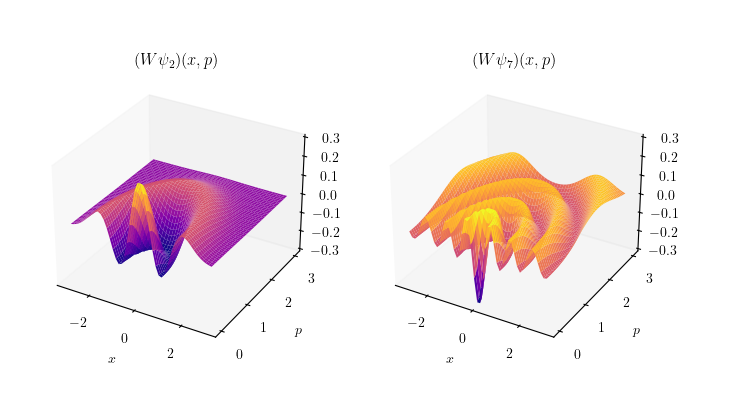
\includegraphics[width=1\textwidth]{imgs/harmonic_osc_wigner.png}
    \caption{Funciones de Wigner de los estados $\psi_3$ y
    $\psi_7$ del oscilador armónico, con $\hbar = 1$ y
    $\omega = 1$.}
    \label{fig:harmonic_osc_wigner_3_7}
  \end{figure}

  \chapter{Funciones de Wigner en el Espacio Fase Discreto}

  Resumiendo el capítulo anterior, tenemos una manera
  distinta a la usual de representar un estado cuántico por
  medio de la transformación de Wigner. Dicha transformación
  nos permite calcular los valores esperados de ciertos
  observables cuánticos, en particular aquellos que su
  símbolo de Weyl está bien definido. Además podemos
  recuperar las densidades probabilísticas de la posición y
  del momentum itegrando la función de Wigner sobre el eje
  de momentum o de posición respectivamente. Ésta última
  característica solamente es un caso partícular de una
  propiedad más general de la función de Wigner.

  \textbf{Operadores puntuales} Podemos utilizar . . .
  FOLLAND
  \begin{equation}
    A(x,p) =
    \Tr\left( \hat{M}(x,p) \Op_W(A) \right),
  \end{equation}
  donde $(\hat{M}(x,p)\psi)(y) = 2e^{2i p (y - x)}\psi(2x -
  y)$. Ésta expresión solo se puede calcular en ciertas
  situaciones, por suerte la que nos interesa calcular es la
  del caso en que $\Op_W(A) = \rho$ es un operador de
  densidad, pues éste es de clase traza.

  \chapter{Construcción no-estándar}

  \newpage
  \appendix

  \chapter{Apéndices}

  \section{Espacio de Schwartz y su dual}

  \begin{definition}
    Sea $\Sz(\R^{n})$ el espacio vectorial complejo
    de las funciones de prueba de Schwartz. La función
    $\psi$ es un elemento de $\Sz(\R^{n})$, si es
    lisa y si las funciones $x^{\beta} \partial_x^{\alpha}
    \psi$ son acotadas para todo los índices $\alpha =
    (\alpha_1, \ldots, \alpha_n)$ y $\beta = (\beta_1,
    \ldots, \beta_n)$ en $\N^{n}$.
  \end{definition}

  \begin{definition}
    El espacio dual de $\Sz(\R^{n})$ es el espacio de
    las distribuciones (ó funciones generalizadas)
    templadas, y lo denotaremos como $\Sz'(\R^{n})$.
  \end{definition}

  \begin{definition}
    El espacio de Hilbert de las (clases de) funciones
    complejas cuadraticamente-integrables sobre $\R^{n}$ se
    denota como $L^2(\R^{n})$, y está equipado con el
    producto interno
    \[
      \langle f, g \rangle
      = \int_{\R^{n}} \overline{f}(x) g(x) \, dx.
    \] 
  \end{definition}
 
  Los elementos del espacio de Schwartz sobre $\R^{n}$
  tienen derivadas parciales que decrecen rápidamente. El
  dual del espacio de Schwartz se conoce como las
  \textit{distribuciones templadas} sobre $\R^{n}$. Existe
  una inclusión natural de las funciones cuadraticamente
  integrables en el espacio de distribuciones. Además, el
  espacio de Schwartz es un subespacio denso de
  $L^2(\R^{n})$, podemos expresar éstas relaciones con un
  poco de abuso de notación,
  \[
    \Sz(\R^{n})
    \subset L^2(\R^{n})
    \subset \Sz'(\R^{n}).
  \]

  Sea $\mathcal D(\R^{n})$ el espacio de las funciones de
  prueba.

  \begin{definition}
    Supongamos que $\{\phi_n\}_{n \in \N}$ es una sucesión
    convergente en $\mathcal D(\R^{n})$ con límite $\phi \in
    \mathcal D(\R^{n})$. Si $T : \mathcal D(\R^{n}) \to \C$
    es un funcional lineal continuo, es decir
    \[
      \forall \psi, \phi \in \mathcal D(\R^{n}) : T(\phi +
      \psi) = T(\phi) + T(\psi),
    \] 
    \[
      \forall \phi \in \mathcal D(\R^{n}) : \forall \alpha
      \in \C : T(\alpha \phi) = \alpha T(\phi),
    \] 
    y
    \[
      \phi_n \to \phi \implies T(\phi_n) \to T(\phi).
    \] 
    Entonces $T$ es una distribución.
  \end{definition}

  \begin{definition}
    Definimos a la distribución de Dirac $\delta_a$ como la
    distribución que satisface
    \[
      \forall \phi \in \mathcal D(\R^{n}) : \delta_a(\phi) =
      \phi(a).
    \] 
  \end{definition}

  $C^{\infty}_0(\R^{n})$ es el conjunto de todas las función
  sobre $\R^{n}$ lisas y con soporte compacto. Los espacios
  $C^{\infty}_0(\R^{n})$ y $\Sz(\R^{n})$ son densos en
  $L^{r}(\R^{n})$, $1 \leq r < \infty$.

  Iniciamos definiendo
  la transformación de Wigner sobre el espacio de las
  funciones de Schwartz $\Sz(\R^{n})$, para ésto primero
  recordamos la transformación de Fourier.

  \begin{definition}
    La transformada de Fourier se denotará por $\F$,
    y usaremos una versión que incluye una constante de
    normalización dada por la constante de Planck,
    \[
      \F\psi(x)
      = \frac{1}{(2\pi\hbar)^{n / 2}} \int_{\R^{n}}
      e^{-\frac{i}{\hbar} x \cdot y} \psi(y) \, dy,
    \] 
    para $\psi \in \Sz(\R^{n})$.
  \end{definition}
  La transformada de Fourier es un automorfismo del espacio
  de Schwartz, y se puede extender a un automorfismo
  unitario sobre $L^2(\R^{n})$, cuya inversa está dada por
  \[
    \F^{-1}\psi(x)
    = \frac{1}{(2\pi\hbar)^{n / 2}} \int_{\R^{n}}
    e^{\frac{i}{\hbar} x \cdot y} \psi(y) \, dy.
  \] 
  Además se puede extender por medio de la dualidad a un
  automorfismo de $\Sz'(\R^{n})$.

  \begin{definition}
    La transformada de Fourier de una función en
    $L^{1}(\R^{n})$ es la función $\hat{f}$ sobre $\R^{n}$ 
    definida como
    \[
      \F[f](\xi) = (2\pi)^{-n / 2} \int_{\R^{n}} e^{-i x
      \cdot \xi} f(x) \, dx, 
      \quad \xi \in \R^{n}.
    \] 
  \end{definition}

  \begin{theorem}
    La transformada de Fourier es biyectiva en
    $\Sz(\R^{n})$.
  \end{theorem}

  \begin{theorem}[Plancherel]
    La biyección $\F : \Sz(\R^{n}) \to \Sz(\R^{n})$ 
    se puede extender únicamente a un operador unitario
    sobre $L^2(\R^{n})$.
  \end{theorem}

  \begin{proposition}
    El espacio $\Sz(\R^{n})$ es denso en $\Sz'(\R^{n})$.
  \end{proposition}

  \section{Wong}

  Sea $f$ una función medible sobre $\R^{n}$. Definimos la
  función $\rho(\xi,\eta)f$ sobre $\R^{n}$ como
  \begin{equation}
    (\rho(\xi,\eta)f)(x)
    = e^{i\xi \cdot x + \frac{1}{2} i \xi \cdot \eta}
    f(x+\eta),
    \quad x \in \R^{n}.
  \end{equation}
  El operador $\rho(\xi,\eta) : L^2(\R^{n}) \to L^2(\R^{n})$
  es unitario para todo $\xi, \eta \in \R^{n}$. Si nos
  enfoncamos en el subespacio de $L^2(\R^{n})$ de las
  funciones de Schwartz, entonces podemos definir la
  siguiente función sobre el espacio de fase $\R^{2n}$. Sean
  $f,g \in \Sz(\R^{n})$, entonces
  \begin{equation}
    V(f,g)(\xi,\eta)
    = (2\pi)^{-n / 2} \langle \rho(\xi,\eta)f, g \rangle.
  \end{equation}
  A ésta función Wong la llama la transformación
  Fourier-Wigner de $f$ y de $g$. De manera explícita
  tenemos 
  \begin{equation}
    V(f,g)(\xi,\eta)
    = (2\pi)^{-n / 2} \int_{\R^{n}} e^{i \xi \cdot y}
    f\left( f + \frac{\eta}{2} \right) \overline{g\left( y -
    \frac{\eta}{2}\right) } \, dy.
  \end{equation}

  El operador $V : \Sz(\R^{n}) \times \Sz(\R^{n}) \to
  \Sz(\R^{2n})$ es un mapeo lineal.

  Wong menciona que la transformada de Wigner $W(f)$ de una
  función en $L^2(\R^{n})$, introducida por Wigner en 1932,
  es una herramienta para el estudio de la distribución de
  probabilidad conjunta no existente de la posición y
  momentum de un estado $f$.

  \begin{theorem}
    Sean $f$ y $g$ elementos de $\Sz(\R^{n})$. Entonces
    \begin{equation}
      \F[V(f,g)](x,\xi)
      = (2\pi)^{-n / 2} \int_{\R^{n}} e^{-i \xi \cdot p
      } f\left( x + \frac{p}{2} \right)
      \overline{g\left( x - \frac{p}{2} \right)} \, dp.
    \end{equation}
  \end{theorem}

  Con ésto Wong define a la transformación de Wigner de dos
  funciones $f$ y $g$ en $\Sz(\R^{n})$ como
  \begin{equation}
    W(f,g)(x,\xi)
    = (2\pi)^{-n / 2} \int_{\R^{n}} e^{-i\xi \cdot p}
    f\left( x + \frac{p}{2} \right) \overline{g\left( x -
    \frac{p}{2} \right) } \, dp.
  \end{equation}

  La transformada de Wigner $W : \Sz(\R^{n}) \times
  \Sz(\R^{n}) \to \Sz(\R^{2n})$ puede ser extendida a un
  operador sesquilineal
  \[
    W : L^2(\R^{n}) \times L^2(\R^{n}) \to L^2(\R^{2n}),
  \] 
  tal que
  \[
    \|W(f,g)\|_{L^2(\R^{2n})}
    = \|f\|_{L^2(\R^{n})} \|g\|_{L^2(\R^{n})}.
  \] 

  De acuerdo a Wong, podemos obtener un operador lineal
  acotado $Q : L^2(\R^{2n}) \to B(L^2(\R^{n}))$ a partir de
  cualquier función $\sigma \in L^2(\R^{2n})$.

  En la mecánica cúantica, los observables deben ser
  representados por operadores auto-adjuntos, la
  transformación de Weyl nos permite hacer ésto.

  La correspondencia resulta ser entre funciones en el
  espacio de fase y los operadores Hilbert-Schmidt.

  \begin{definition}
    Sea $h \in L^2(\R^{2n})$. Definimos el operador $S_h :
    L^2(\R^{n}) \to L^2(\R^{n})$ como
    \begin{equation}
      (S_hf)(x)
      = \int_{\R^{n}} h(x,y) f(y) \, dy,
    \end{equation}
    para todo $f \in L^2(\R^{n})$.
  \end{definition}
  Al operador $S_h$ se le conoce como el operador
  Hilbert-Schmidt correspondiente al núcleo $h$.

  Para probar que el conjunto de transformaciones de Weyl
  con símbolos en $L^2(\R^{2n})$ es igual al conjunto de
  operadores Hilbert-Schmidt sobre $L^2(\R^{n})$, Wong
  define y utiliza el producto tensorial de funciones de
  $L^2(\R^{n})$.

  \begin{theorem}
    Sea $\sigma \in L^2(\R^{2n})$. Entonces $W_\sigma :
    L^2(\R^{n}) \to L^2(\R^{n})$ es un operador
    Hilbert-Schmidt con núcleo $(2\pi)^{-n / 2}K \sigma$
    donde $K : L^2(\R^{2n}) \to L^2(\R^{2n})$ se define como
    \[
      (Kf)(x,y)
      = (T^{-1}\F_2 f)(y,x).
    \] 
  \end{theorem}

  Entonces ahora sabemos que si $\sigma \in L^2(\R^{2n})$,
  entonces $W_\sigma$ es un operador Hilbert-Schmidt con
  núcleo $(2\pi)^{-n / 2} K \sigma$. El converso es cierto
  también, si $A$ es un operador Hilbert-Schmidt arbitrario,
  entonces tiene un representación integral $A = S_h$, y
  $\sigma = (2\pi)^{-n / 2} K^{-1}h$.

  Se puede definir la transformación de Weyl para símbolos
  en $\Sz'(\R^{2n})$. Resulta que para $2 < r < \infty$,
  existe una función $\sigma \in L^{r}(\R^{2n})$ tal que la
  transformación de Weyl $W_\sigma$ no es un operador lineal
  acotado sobre $L^2(\R^{n})$.

  \section{Resumen de Folland}

  Para Folland, la transformación de Wigner de dos funciones
  $f$ y $g$ es la transformación de Fourier de la
  transformación de Fourier-Wigner:
  \[
    W(f,g)(\xi, \eta)
    = \int_{\R^{2n}} e^{-2\pi i (\xi q + \eta p} V(f,g)(q,x)
    \, dp \, dq.
  \] 
  Donde
  \[
    V(f,g)(q,p)
    = \int e^{2\pi i q y} f(y + \frac{1}{2}p)\overline{g(y -
    \frac{1}{2}p)} \, dy.
  \] 
  Así que
  \[
    W(f,g)(\xi, \eta) = \int e^{-2\pi i \eta p }
    f(x+\frac{1}{2}p)\overline{g(y-\frac{1}{2}p)} \, dp.
  \] 

  Folland muestra que $W$ mapea $\Sz(\R^{n}) \times
  \Sz(\R^{n})$ a $\Sz(\R^{2n})$ y se puede extender al caso
  de las distribuciones templadas.

  \newpage
  \printbibliography

\end{document}
